
\chapter{Revisão de literatura}

\section{\emph{Solanum Lycopersicum L.}}
Lorem ipsum dolor sit amet, consectetur adipiscing elit. Vestibulum sem lectus, vestibulum et semper sit amet, sodales vitae est. Nulla euismod facilisis elementum. Sed non dictum eros, nec malesuada lacus. Praesent ut efficitur mauris. Donec porttitor mattis euismod. Suspendisse tristique lacus lectus, semper dapibus tortor dapibus ac. Donec fermentum leo id erat sagittis porta. Aenean nec pellentesque dui, ac pellentesque diam. Phasellus placerat, augue vitae tincidunt lobortis, risus diam auctor enim, et efficitur nisl dui interdum metus. Nam sapien ligula, porta vitae posuere in, feugiat at massa. In vel sodales enim.

Phasellus volutpat condimentum quam, sed ultrices velit. Duis malesuada tincidunt tempus. Aliquam lectus purus, semper quis ante in, rhoncus convallis quam. Maecenas ex neque, aliquet sit amet lobortis vitae, blandit quis purus. Aliquam aliquam quam vel rhoncus placerat. Duis nulla neque, euismod ac pharetra non, tempor eu quam. Nulla sollicitudin, risus in vestibulum ullamcorper, dolor justo suscipit nisl, at luctus nunc ex eget neque. Maecenas quis felis sapien. Vivamus tempor et neque sit amet dignissim. Aliquam pulvinar turpis in tortor ultrices ornare. Etiam ultricies vel sapien vitae gravida.

Donec lorem velit, commodo in convallis eu, tristique eu dui. Donec bibendum leo mi, non consequat arcu aliquet ut. Ut consectetur lacus eros, nec efficitur sem faucibus a. Donec sit amet nulla facilisis, euismod libero eget, auctor nisl. Pellentesque habitant morbi tristique senectus et netus et malesuada fames ac turpis egestas. Vestibulum vitae massa quis ante malesuada tristique. Praesent posuere enim non urna convallis hendrerit. Vestibulum neque ligula, varius quis vehicula ut, lacinia vitae eros. Curabitur at lectus sagittis, tempus nunc ac, maximus massa. Pellentesque vehicula, eros tincidunt accumsan ultricies, elit diam cursus leo, eget dapibus sem orci non neque. Vivamus auctor erat ac metus imperdiet, ut sagittis justo dapibus.

Ut dapibus elit sed elementum maximus. Praesent maximus convallis lacus, vitae tempor purus euismod et. Donec elementum id dui vel aliquet. Maecenas at convallis est, at faucibus nisi. Aliquam quis euismod lorem. Vivamus in ex a diam vehicula finibus. Sed venenatis vitae risus eget fermentum. Nunc ullamcorper neque id dolor porta, in fringilla diam lobortis.

Cras vehicula venenatis augue, et venenatis eros feugiat sit amet. Duis tellus urna, eleifend quis erat sed, elementum euismod elit. Donec vel ex luctus, porttitor erat sit amet, malesuada lectus. Cras at nisi ligula. Vestibulum sit amet ullamcorper tortor. Suspendisse potenti. Nam vehicula turpis ante, id aliquet ante varius non.


\section{Considerações iniciais sobre o Biospeckle}

%%%%%%%%%%%%%%%%%%%%%%%%%%%%%%% exemplo de Figúra%%%%%%%%%%%%%%%%

\begin{figure}[!htb]
	\caption{Imagens de STS sem atividade e com alta atividade respectivamente.
}
  \centering
  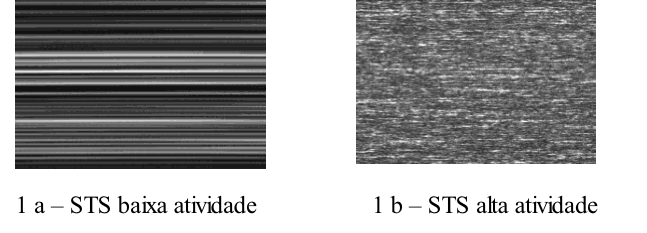
\includegraphics[scale=1.0]{Imagens/imagem_1.png} 
  \legend{Fonte: \cite{enes_alise_2006}}
  \label{figura0}
\end{figure}

% %Com o newpage vou forçar a descrição ficar na próxima página
Lorem ipsum dolor sit amet, consectetur adipiscing elit. Vestibulum sem lectus, vestibulum et semper sit amet, sodales vitae est. Nulla euismod facilisis elementum. Sed non dictum eros, nec malesuada lacus. Praesent ut efficitur mauris. Donec porttitor mattis euismod. Suspendisse tristique lacus lectus, semper dapibus tortor dapibus ac. Donec fermentum leo id erat sagittis porta. Aenean nec pellentesque dui, ac pellentesque diam. Phasellus placerat, augue vitae tincidunt lobortis, risus diam auctor enim, et efficitur nisl dui interdum metus. Nam sapien ligula, porta vitae posuere in, feugiat at massa. In vel sodales enim.



%%%%%%%%%%%%%%%%%%%%%%%%% Equação%%%%%%%%%%%%%%%%
\begin{equation} \label{eq:01}
CON = \left | Nij \right |
\end{equation}


em que,

\textbf{Nij} – número de ocorrências de intensidades
\textbf{i,j} – intensidades sucessivas

Lorem ipsum dolor sit amet, consectetur adipiscing elit. Vestibulum sem lectus, vestibulum et semper sit amet, sodales vitae est. Nulla euismod facilisis elementum. Sed non dictum eros, nec malesuada lacus. Praesent ut efficitur mauris. Donec porttitor mattis euismod. Suspendisse tristique lacus lectus, semper dapibus tortor dapibus ac. Donec fermentum leo id erat sagittis porta. Aenean nec pellentesque dui, ac pellentesque diam. Phasellus placerat, augue vitae tincidunt lobortis, risus diam auctor enim, et efficitur nisl dui interdum metus. Nam sapien ligula, porta vitae posuere in, feugiat at massa. In vel sodales enim.Lorem ipsum dolor sit amet, consectetur adipiscing elit. Vestibulum sem lectus, vestibulum et semper sit amet, sodales vitae est. Nulla euismod facilisis elementum. Sed non dictum eros, nec malesuada lacus. Praesent ut efficitur mauris. Donec porttitor mattis euismod. Suspendisse tristique lacus lectus, semper dapibus tortor dapibus ac. Donec fermentum leo id erat sagittis porta. Aenean nec pellentesque dui, ac pellentesque diam. Phasellus placerat, augue vitae tincidunt lobortis, risus diam auctor enim, et efficitur nisl dui interdum metus. Nam sapien ligula, porta vitae posuere in, feugiat at massa. In vel sodales enim.

\begin{equation} \label{eq:02}
MDI = \sum_{ij} M ij(i-j)^{2}
\end{equation}

\section{Análise de frequência do Biospeckle laser}


\subsection{A transformada de Fourier}

Lorem ipsum dolor sit amet, consectetur adipiscing elit. Vestibulum sem lectus, vestibulum et semper sit amet, sodales vitae est. Nulla euismod facilisis elementum. Sed non dictum eros, nec malesuada lacus. Praesent ut efficitur mauris. Donec porttitor mattis euismod. Suspendisse tristique lacus lectus, semper dapibus tortor dapibus ac. Donec fermentum leo id erat sagittis porta. Aenean nec pellentesque dui, ac pellentesque diam. Phasellus placerat, augue vitae tincidunt lobortis, risus diam auctor enim, et efficitur nisl dui interdum metus. Nam sapien ligula, porta vitae posuere in, feugiat at massa. In vel sodales enim.

\begin{equation} \label{eq:03}
F(w)=\int_{-\infty }^{\infty} f(t)e^{-wt} dt
\end{equation}



%%%%%%%%%%%%%%% Exemplo de código%%%%%%%%%%
\begin{listing}[H]
    \caption{Trecho código para divisão em Frames}
    \label{labelFrame}
	\begin{minted}{MATLAB}
    for img = 1:128;
    filename=strcat('seed',num2str(img),'.bmp'); 
    frame2 = read(a, img);
    img2 = uint8(frame2(1:480,1:640));
    imwrite(img2,filename);
	\end{minted}
	\label{cod2}

\end{listing}


